% !Mode:: "TeX:UTF-8"
\documentclass[QA.tex]{subfiles}

\begin{document}
%-=-=-=-=-=-=-=-=-=-=-=-=-=-=-=-=-=-=-=-=-=-=-=-=
%
%	CHAPTER
%
%-=-=-=-=-=-=-=-=-=-=-=-=-=-=-=-=-=-=-=-=-=-=-=-=

%%================================================================
\chapter{20171102}\label{ch1102}
%----------------------------------------------------------------------------------------

\begin{qst}\label{Q2017110201}
左引号显示不对,怎么办?\index{左引号}
\end{qst}
\ans 用反撇号\verb|`|。或者直接用 unicode。

\begin{qst}\label{Q2017110202}
这样的矩阵该怎么输入呢,求大神赐教。

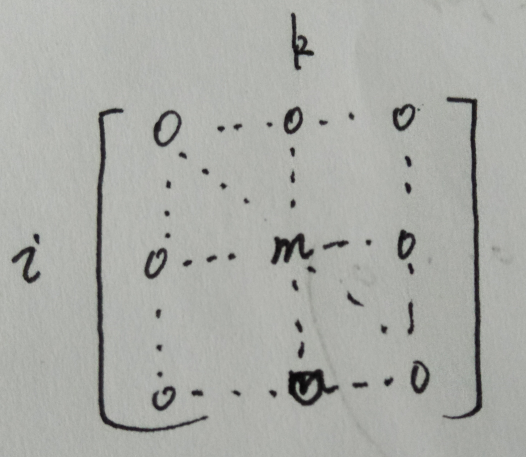
\includegraphics[width=0.85\textwidth]{pic02.png}
\end{qst}
\ans 可以一个三阶矩阵套一个三阶矩阵,
\[
\begin{matrix}
&	i&	\\
j&	\left[ \begin{matrix}
0&	\cdots&	0&	\cdots&	0\\
\vdots&	\ddots&	\vdots&	&	\vdots\\
0&	\cdots&	m&	\cdots&	0\\
\vdots&	&	\vdots&	\ddots&	\vdots\\
0&	\cdots&	0&	\cdots&	0\\
\end{matrix} \right]&
\end{matrix}
\]
\begin{verbatim}
\[
\begin{matrix}
&	i&	\\
j&	\left[ \begin{matrix}
0&	\cdots&	0&	\cdots&	0\\
\vdots&	\ddots&	\vdots&	&	\vdots\\
0&	\cdots&	m&	\cdots&	0\\
\vdots&	&	\vdots&	\ddots&	\vdots\\
0&	\cdots&	0&	\cdots&	0\\
\end{matrix} \right]&
\end{matrix}
\]
\end{verbatim}

也可以二阶矩阵套三阶矩阵。
\[
\begin{matrix}
&i\\
j&\left[ \begin{matrix}
0&\cdots&0&\cdots&0\\
\vdots&\ddots&\vdots&&\vdots\\
0&\cdots&m&\cdots&0\\
\vdots&&\vdots&\ddots&\vdots\\
0&\cdots&0&\cdots&0\\
\end{matrix} \right]
\end{matrix}
\]
\begin{verbatim}
\[
\begin{matrix}
&i\\
j&\left[ \begin{matrix}
0&\cdots&0&\cdots&0\\
\vdots&\ddots&\vdots&&\vdots\\
0&\cdots&m&\cdots&0\\
\vdots&&\vdots&\ddots&\vdots\\
0&\cdots&0&\cdots&0\\
\end{matrix} \right]
\end{matrix}
\]
\end{verbatim}

还可以用边界矩阵环境 bordermatrix。\index{边界矩阵}
\[
\bordermatrix{
	&	     &        & i      &		&        \cr
	& 0      & \cdots & 0      & \cdots & 0      \cr
	& \vdots & \ddots & \vdots &		& \vdots \cr
  j & 0      & \cdots & m      & \cdots & 0      \cr
	& \vdots &		  & \vdots & \ddots & \vdots \cr
	& 0      & \cdots & 0      & \cdots & 0
}
\]
\begin{verbatim}
\[
\bordermatrix{
	&	     &        & i      &		&        \cr
	& 0      & \cdots & 0      & \cdots & 0      \cr
	& \vdots & \ddots & \vdots &		& \vdots \cr
  j & 0      & \cdots & m      & \cdots & 0      \cr
	& \vdots &		  & \vdots & \ddots & \vdots \cr
	& 0      & \cdots & 0      & \cdots & 0
}
\]
\end{verbatim}

可以参考\url{http://blog.sina.com.cn/s/blog_5e16f1770102dqp2.html}.

\begin{qst}\label{Q2017110203}
发现latex2e sources里面对于很多标准宏包的好多参数和尺寸说明的相当详细,
 对于想修改那些常见命令环境或者作为参考很有帮助。
命令行运行texdoc source2e即可打开。
虽说那个latex2e sources有不少源码,不过看起来也不费劲,排的算是很精校了。

\end{qst}
\ans 那个是用 docstrip 宏包排版的,专门处理代码和注释。

\begin{qst}\label{Q2017110204}
在\LaTeX{}中,表格与上下方文字距离过大怎么调整!
\end{qst}
\ans 试试array宏包的\verb|\extratabsurround|,设置一下合适的间距。\index{extratabsurround}

\begin{qst}\label{Q2017110205}
请问word的小四、五号字对应LaTeX多少pt呢?\index{字号}
\end{qst}
\ans 铅字时代的小四和五号是12pt和10.5pt。
word时代就是把上面的pt换成bp。

\begin{qst}\label{Q2017110206}
有没有人知道如何把代码统一缩进啊?用的lstlisting。\index{代码缩进}
\end{qst}
\ans 你去看文档就知道 listings 有个 basic style的设置。比如
\begin{verbatim}
\lstset{% general command to set parameter(s)
basicstyle=\ttfamily\fontsize{9pt}{12pt}\selectfont,
keywordstyle=\color{blue}\bfseries,
commentstyle=\color{gray},
showstringspaces=false,
xleftmargin=1cm}
\end{verbatim}

\begin{qst}\label{Q2017110207}
单双栏混排通栏公式怎么搞?\index{通栏公式}
\end{qst}
\ans 有 widetext 和 cuted 两个宏包可供选择。
单栏公式可以,但顺序还是不行。
这个帖子讨论了类似的问题\url{http://latex.org/forum/viewtopic.php?t=2770}.

\begin{qst}{Q2017110208}
如图的双箭头如何更换箭头形状?\index{箭头形状}

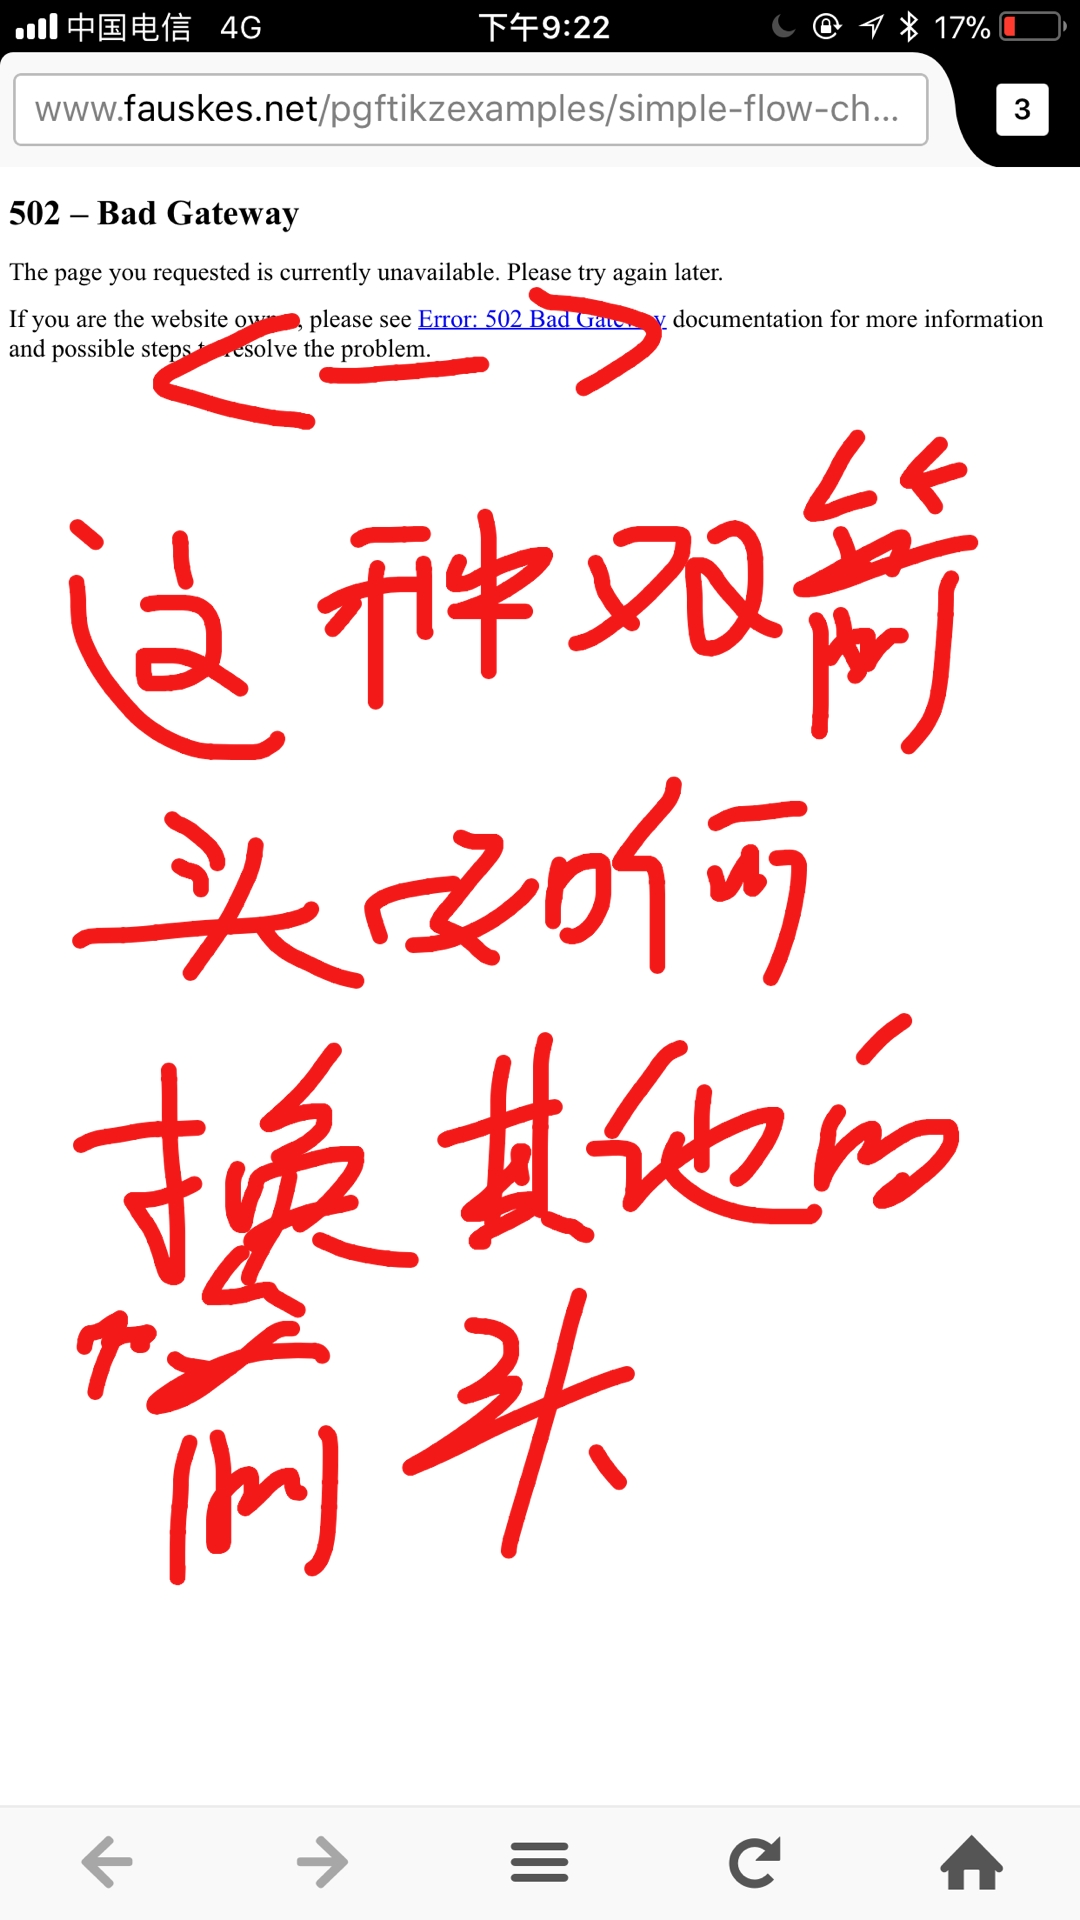
\includegraphics[width=0.35\textwidth]{pic03.jpg}
\end{qst}
\ans 可以直接选择合适的指令,比如

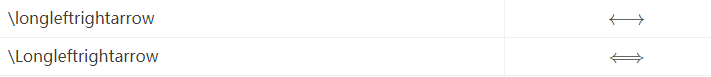
\includegraphics[width=0.65\textwidth]{pic04.png}

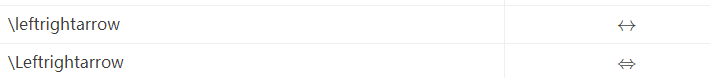
\includegraphics[width=0.65\textwidth]{pic05.png}


\includegraphics[width=0.65\textwidth]{pic06.png}

使用Tikz绘图时可以指定箭头形状。

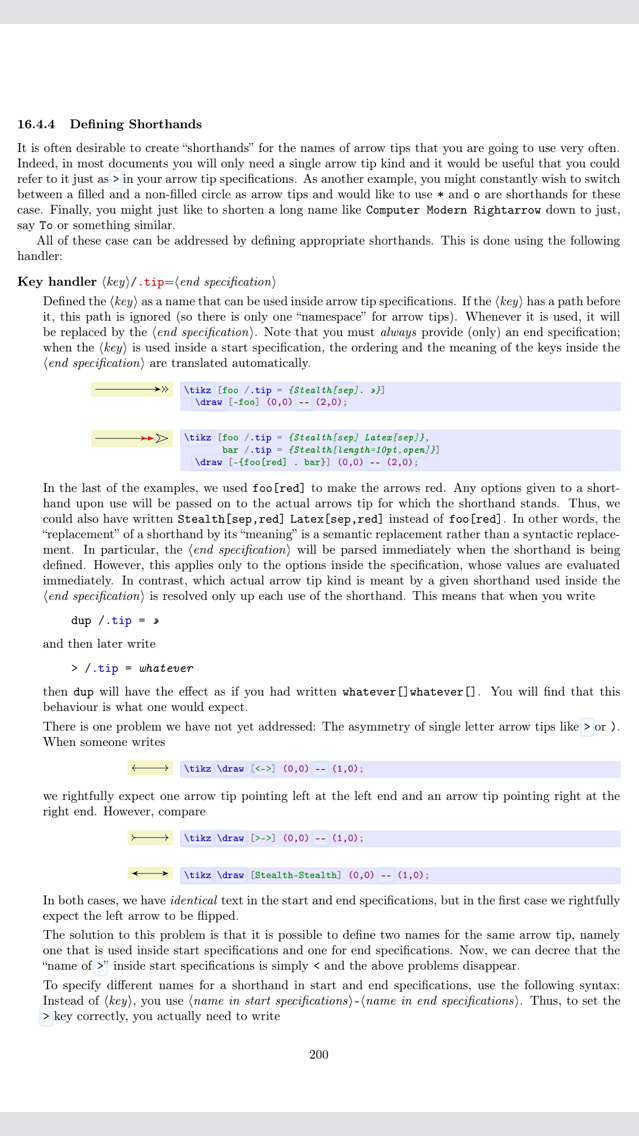
\includegraphics[width=0.45\textwidth]{pic07.png}
\end{document} 